\documentclass{article}

\usepackage{graphicx}
\usepackage{tikz}
\usepackage{tikzsymbols}
\usetikzlibrary{calc,patterns,shapes.geometric}
\pagestyle{empty}
\usepackage[margin=0pt]{geometry}
\geometry{papersize={14in,12in}}

\def\centerarc[#1](#2)(#3:#4:#5){\draw[#1] ($(#2)+({#5*cos(#3)},{#5*sin(#3)})$) arc (#3:#4:#5);}

\begin{document}
	\begin{figure}
		\centering
		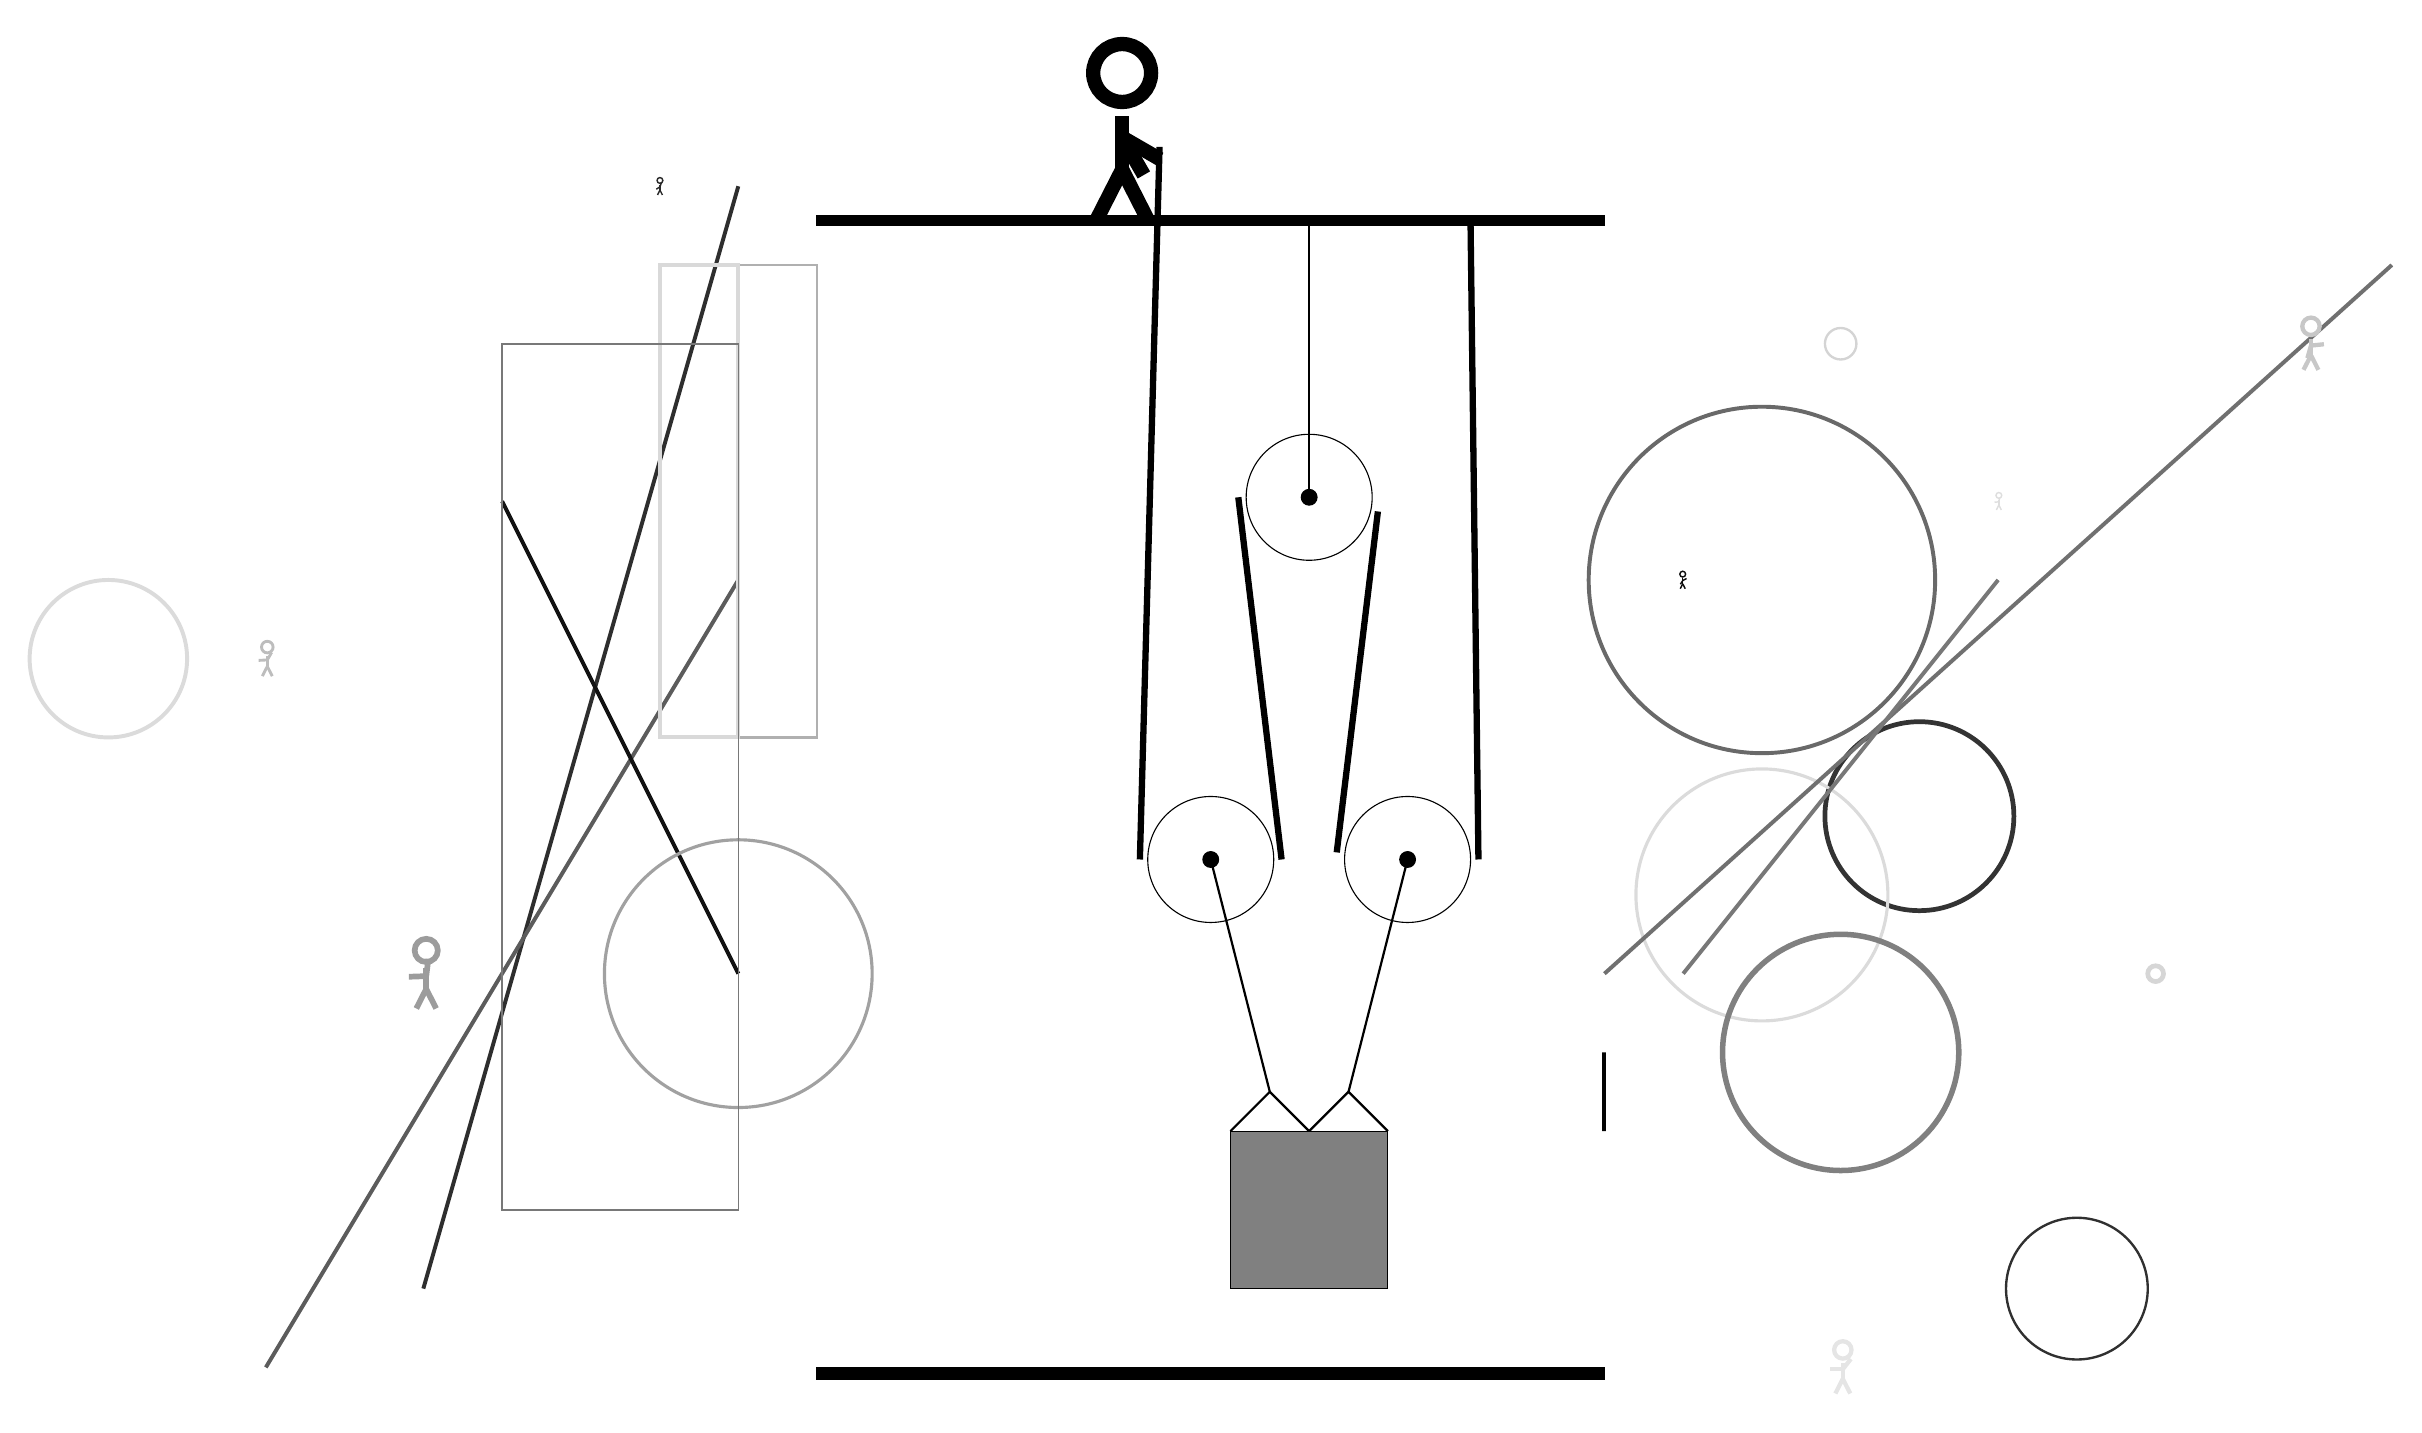
\begin{tikzpicture}
			%%%%% START %%%%%
			
			\draw[fill=black] (-4, 11.5) rectangle (6, 11.625);
			
			\draw (1, 3.45) circle (0.8);
			\draw[fill=black] (1, 3.45) circle (0.1);
			
			\draw (2.25, 8.05) circle (0.8);
			\draw[fill=black] (2.25, 8.05) circle (0.1);
			\draw[thick] (2.25, 8.05) -- (2.25, 11.5);
			
			\draw (3.5, 3.45) circle (0.8);
			\draw[fill=black] (3.5, 3.45) circle (0.1);
			
			\draw[thick] (3.5, 3.45) -- (2.75, 0.5);
			\draw[thick] (1, 3.45) -- (1.75, 0.5);
			\draw[thick]  (1.25, 0) -- (1.75, 0.5) -- (2.25, 0);
			\draw[thick]  (2.25, 0) -- (2.75, 0.5) -- (3.25, 0);
			\draw[fill=black!50] (1.25, 0) rectangle (3.25, -2);
			
			\draw[line width=0.8mm] (0.35, 12.5) --  (0.1, 3.45);
			\centerarc[line width=0.8mm](1, 3.45)(180:360:0.9);
			\draw[line width=0.8mm] (1.9, 3.45) -- (1.35, 8.05);
			\centerarc[line width=0.8mm](2.25, 8.05)(-20:180:0.9);
			\draw[line width=0.8mm](3.123, 7.87) -- (2.6, 3.54);
			\centerarc[line width=0.8mm](3.5, 3.45)(160:360:0.9);
			\draw[line width=0.8mm](4.4, 3.45) -- (4.3, 11.5);
			
			\node at (-0.07, 12.7) {\Strichmaxerl[10][120][-30]};
			
			\draw[line width=0.5mm, color=black!82](-5, 12) -- (-9, -2);
			
			\draw [line width=0.6mm, color=black!80](10, 4) circle (1.2);
			\draw [line width=0.4mm, color=black!14](8, 3) circle (1.6);
			\draw[line width=0.5mm, color=black!99] (6, 1) rectangle (6, 0);
			
			\draw [line width=0.6mm, color=black!16](13, 2) circle (0.1);
			\draw[line width=0.5mm, color=black!64](-5, 7) -- (-11, -3);
			\draw [line width=0.5mm, color=black!59](8, 7) circle (2.2);
			\node[line width=0.6mm, color=black!26] at (-11, 6) {\Strichmaxerl[2][3][60]};
			\node[line width=0.2mm, color=black!10] at (9, -3) {\Strichmaxerl[3][0][52]};
			\draw [line width=0.5mm, color=black!14](-13, 6) circle (1.0);
			\draw [line width=0.7mm, color=black!50](9, 1) circle (1.5);
			
			\draw[line width=0.5mm, color=black!93](-5, 2) -- (-8, 8);
			\draw[line width=0.3mm, color=black!31] (-6, 11) rectangle (-4, 5);
			
			\draw[line width=0.5mm, color=black!56](6, 2) -- (16, 11);
			\draw [line width=0.3mm, color=black!17](9, 10) circle (0.2);
			\node[line width=0.3mm, color=black!84] at (-6, 12) {\Strichmaxerl[1][32][71]};
			\draw[line width=0.5mm, color=black!53](7, 2) -- (11, 7);
			\node[line width=0.6mm, color=black!13] at (11, 8) {\Strichmaxerl[1][5][79]};
			\draw[line width=0.6mm, color=black!51] (-5, 6) rectangle (-5, 6);
			
			\draw [line width=0.3mm, color=black!81](12, -2) circle (0.9);
			\node[line width=0.4mm, color=black!39] at (-9, 2) {\Strichmaxerl[4][2][83]};
			
			\draw[line width=0.5mm, color=black!15] (-5, 5) rectangle (-6, 11);
			
			\draw [line width=0.4mm, color=black!37](-5, 2) circle (1.7);
			\draw[line width=0.2mm, color=black!53] (-5, 10) rectangle (-8, -1);
			\node[line width=0.2mm, color=black!22] at (15, 10) {\Strichmaxerl[3][74][6]};
			
			\node[line width=0.3mm, color=black!95] at (7, 7) {\Strichmaxerl[1][57][28]};
			
			
			\draw[fill=black] (-4, -3) rectangle (6, -3.15);
			
			%%%%% END %%%%%
		\end{tikzpicture}
	\end{figure}	
\end{document}